Consider the $2\times3$ rectangle below. We fill in the small squares with the numbers $1,2,3,4,5,6$ (one per square). Define a \emph{tasty} filling to be one such that each row is \textbf{not} in numerical order from left to right and each column is \textbf{not} in numerical order from top to bottom. If the probability that a randomly selected filling is tasty is $\frac{m}{n}$ for relatively prime positive integers $m$ and $n$, what is $m+n$?
\begin{center}
	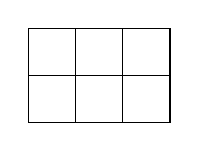
\begin{tikzpicture}[scale=0.6]
		\draw (0,0)--(3,0)--(3,2)--(0,2)--cycle;
		\draw (0,1)--(3,1);
		\draw (1,0)--(1,2);
		\draw (2,0)--(2,2);
	\end{tikzpicture}
\end{center}